\section{Optimising the Time-Response Using Root Locus}

\begin{questions}
\setcounter{question}{\value{lastquestioncounter}}

\question[1M]
Calculate the positions of the open-loop zeros (ie the zeros of $C(s)H(s)$) for the values of $l$, $m$, $K_P$, $K_I$ and $K_D$ that you have used.

\begin{solution}
   Multiplying $C(s)$ which is Eq (\ref{eq:TF_of_PID}) and $H(s)$ which is Eq (\ref{eq:TF_of_Segway}) yields
   \begin{equation}\label{eq:C(s)H(s)}
   \begin{split}
   C(s)H(s) &= \frac{K_D s^2 + K_P s + K_I}{s} \frac{1}{m s^2 - \frac{g}{l}} \\
   &= \frac{K_D s^2 + K_P s + K_I}{m s^3 - \frac{g}{l} s}
   \end{split}
   \end{equation}

   Zeros is the roots of $C(s)H(s)$'s numerator
   \begin{align*}
   Zeros &= \frac{-K_P \pm \sqrt{K^2_P - 4 K_D K_I}}{2 K_D} \\
   &= -0.9186 \pm 0.3951j
   \end{align*}
\end{solution}

\question[2E]
State the positions of the open-loop poles (ie the poles of $C(s)H(s)$) for the values of $l$ and $m$ that you have used.

\begin{solution}
   Poles is the roots of $C(s)H(s)$'s denominator
   \begin{align*}
   Poles &= 0, \pm \sqrt{\frac{g}{lm}} \\
   &= 0, \pm 0.1542
   \end{align*}
\end{solution}

\newpage
\question[3M]
Sketch the root locus for $C(s)H(s)$ and identify the points on the root locus that are such that $Re(s) = \frac{-4}{t_s}$.

\begin{solution}
   \fullwidth{\textbf{Open-loop poles and zeros}}

   They have been calculated in the previous questions:
   \begin{itemize}
      \item zeors at $-0.9186 \pm 0.3951$
      \item poles at $0$, $\pm 0.1542$
   \end{itemize}

   \fullwidth{\textbf{Real-axis segments}}

   \begin{minipage}[htbp]{\linewidth}
      \centering
      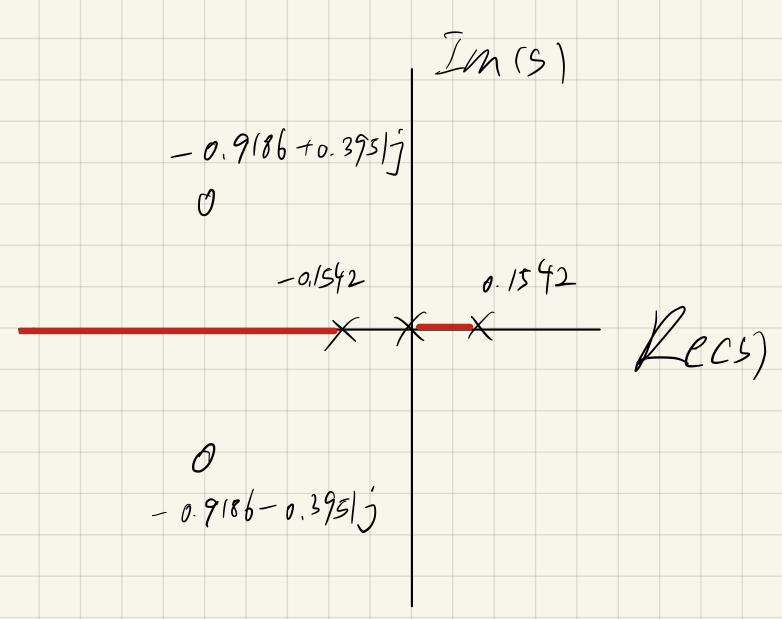
\includegraphics[scale=0.67]{figures/real_axis_segments.png}
      \captionof{figure}{Read lines are real axis segments}
   \end{minipage}

   \fullwidth{\textbf{Infinite poles and zeros}}

   There are three poles and two zeros; therefore, need one infinite zero such that the number of poles and zeros are balanced.

   \fullwidth{\textbf{Asymptotes}}

   The asymptotes touch the real axis at
   \begin{equation*}
   \begin{split}
   \sigma_a &= \frac{\sum_{i=1}^{m} p_i - \sum_{i=1}^{n} z_i}{m-n} \\
   &= \frac{0 + 0.1542 - 0.1542 - (-0.9186 + 0.3951j + -0.9186 - 0.3951j)}{3-2} \\
   &= 1.8372
   \end{split}
   \end{equation*}

   The angle of asymptote(s) is
   \begin{equation*}
   \begin{split}
   \theta_a &= \frac{(2k+1)\pi}{m-n},\ \text{where}\ k \in \{0,1,2,3,\ldots,\infty\}\\
   &= \frac{(2k+1)\pi}{3-2} \\
   &= (2k+1)\pi \\
   &= \pi\ rad
   \end{split}
   \end{equation*}

   \fullwidth{\textbf{Real-axis breakaway points}}

   \begin{align}
   1 + K C(s)H(s) &= 0 \nonumber\\
   K C(s)H(s) &= -1 \nonumber\\
   \because K &\geq 0 \nonumber\\
   \therefore K &= \frac{1}{|C(s)H(s)|} \label{eq:K}
   \end{align}

   K is a local maximum or minimum when root locus breaks away from the real axis; therefore the breakaway points satisfiy
   \begin{equation*}
   \frac{d}{ds} K = 0
   \end{equation*}

   Substituting Eq (\ref{eq:K}) and Eq (\ref{eq:C(s)H(s)})
   \begin{equation*}
   \frac{d}{ds} \frac{1}{\frac{K_D s^2 + K_P s + K_I}{m s^3 - \frac{g}{l} s}} = 0
   \end{equation*}

   and solve it by MATLAB, the breakaway points are
   \begin{equation*}
   s =
   \begin{bmatrix}
    0.0844 \\
   -0.0941 \\
   -1.2310 \\
   -2.4338 \\
   \end{bmatrix}
   \end{equation*}

   \newpage
   \begin{minipage}[htbp]{\linewidth}
      \centering
      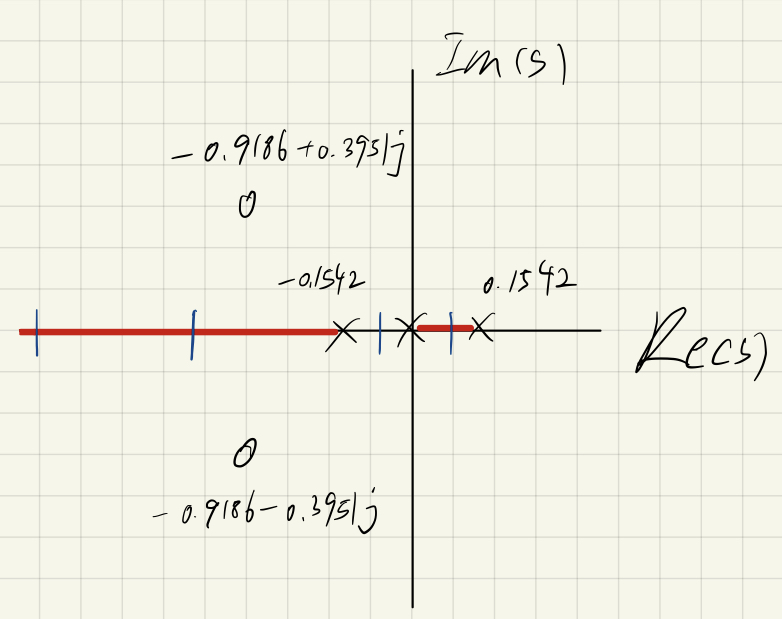
\includegraphics[scale=0.7]{figures/breakaway_points.png}
      \captionof{figure}{Blue vertical lines mark all possible breakaway points}
      \label{fig:breakaway_points}
   \end{minipage}

   However, as shown in Figure \ref{fig:breakaway_points}, $-0.0941$ does not sit on the route locus, so it should not be considered as a breakaway point; hence there are three breakaway point:
   \begin{equation*}
   s =
   \begin{bmatrix}
    0.0844 \\
   -1.2310 \\
   -2.4338 \\
   \end{bmatrix}
   \end{equation*}

   In summary, there are one infinite zero, one asymptote which touches 1.8372 at the real axis and has $\pi$ rad points to the infinite zero, and three breakaway points which are $0.0844$, $-1.2310$, and $-2.4338$.

   \fullwidth{\textbf{Sketch root locus}}

   \begin{minipage}[htbp]{\linewidth}
      \centering
      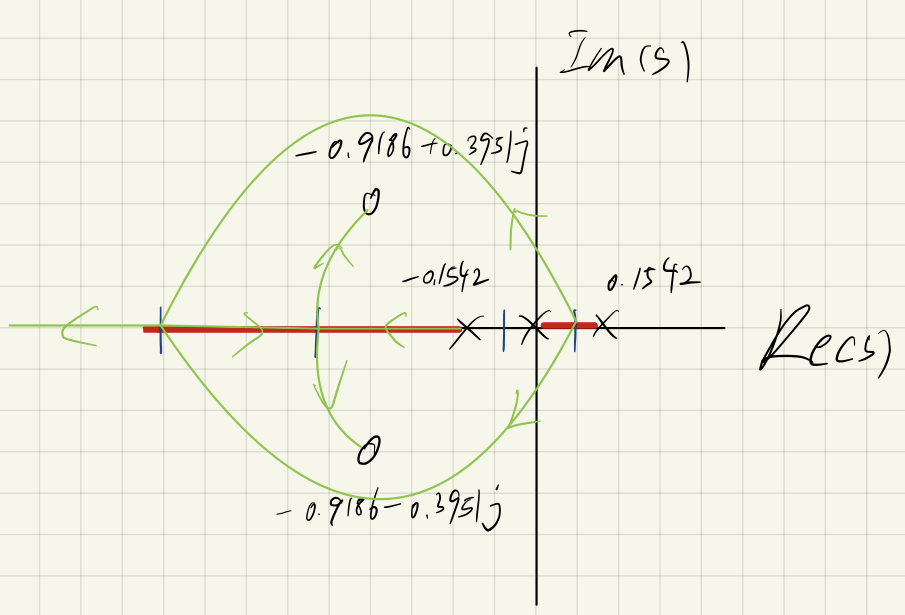
\includegraphics[scale=0.62]{figures/root_locus.png}
      \captionof{figure}{Green lines are root locus}
   \end{minipage}

   \fullwidth{\textbf{Identify the points on the root locus that are
   such that $Re(s) = \frac{-4}{t_s}$}}

   \begin{equation}\label{eq:Re(s)}
   \begin{split}
   Re(s) &= -\frac{4}{t_s} \\
   &= -\frac{4}{8} \\
   &= -0.5
   \end{split}
   \end{equation}

   \begin{minipage}[htbp]{\linewidth}
      \centering
      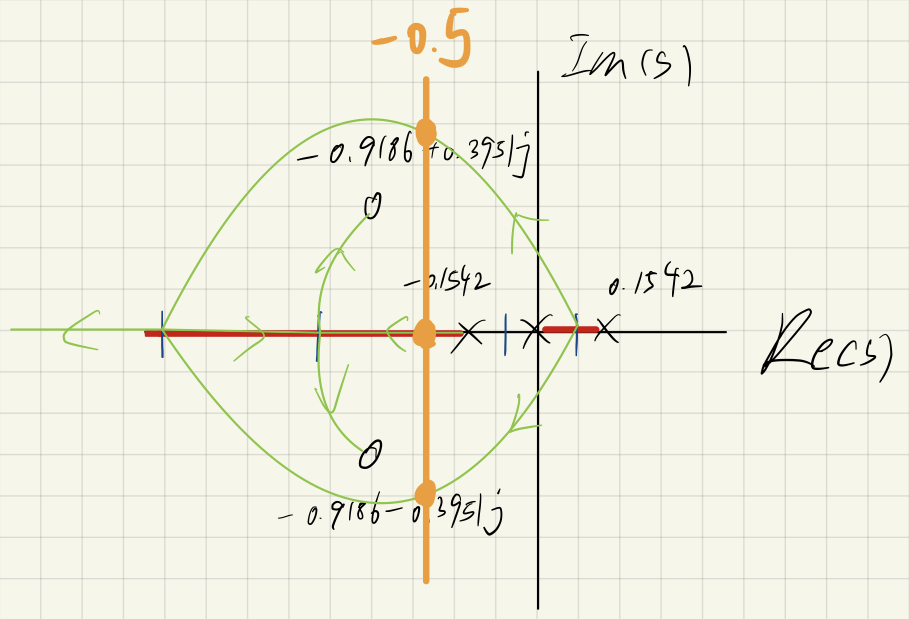
\includegraphics[scale=0.55]{figures/-0.5.png}
      \captionof{figure}{Points on the root locus that are
      such that $Re(s) = -0.5$}
   \end{minipage}

   \fullwidth{\textbf{Validate the sketch via MATLAB}}

   \begin{minted}[fontsize=\small, xleftmargin=-20pt]{matlab}
   m = 12; l = 13; g = 3.711;
   K_P = 132.285; K_D = 72; K_I = 72;
   CH = tf([K_D K_P K_I], [m 0 -g/l 0])
   rlocus(CH)
   \end{minted}
   \begin{minipage}[htbp]{\linewidth}
      \centering
      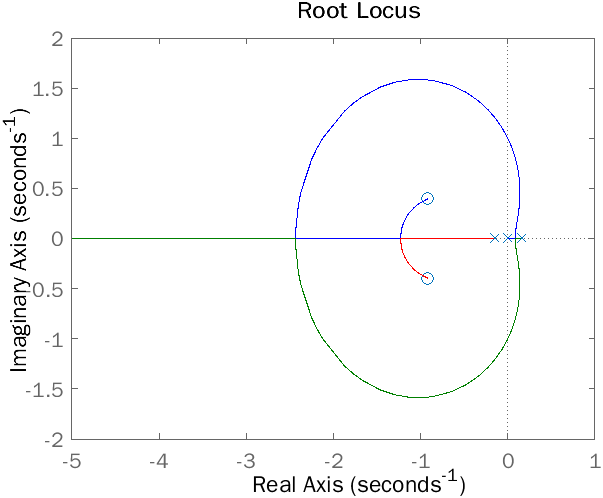
\includegraphics[scale=0.7]{figures/root_locus_matlab.png}
      \captionof{figure}{Root locus from MATLAB}
   \end{minipage}

\end{solution}

\question[1H]
Write the open-loop transfer function, $C(s)H(s)$, as a ratio of polynomials in $s$.

\begin{solution}
   \begin{equation}\label{eq: C(s)H(s) with values}
   C(s)H(s) = \frac{72s^2 + 132.3s + 72}{12s^3 - 0.2855s}
   \end{equation}
\end{solution}

\question[1H]
Write $P(s) + KZ(s) = 0$ as a polynomial in $s$ involving $K$.

\begin{solution}
   $P(s)$ is the denominator of the fraction (\ref{eq: C(s)H(s) with values})
   \begin{equation*}
   P(s) = 12s^3 - 0.2855s
   \end{equation*}

   $Z(s)$ is the numerator of the fraction (\ref{eq: C(s)H(s) with values})
   \begin{equation*}
   Z(s) = 72s^2 + 132.3s + 72
   \end{equation*}

   Sub $P(s)$ and $Z(s)$ into $P(s) + KZ(s) = 0$ and rearrange to the polynominal form
   \begin{equation}\label{eq:P(s)+KZ(s)=0}
   13s^3 + 72Ks^2 + (132.3K-0.2855)s + 72K = 0
   \end{equation}
\end{solution}

\question[1H]
Write $P(\tilde{s})+KZ(\tilde{s}) = 0$ as a polynomial in $\tilde{s}$ involving $K$.

\begin{solution}
   Sub $s = \tilde{s} - Re(s)$, where $Re(s)$ has been evaluated at (\ref{eq:Re(s)}), into Eq (\ref{eq:P(s)+KZ(s)=0}) yields
   \begin{equation*}
   12\tilde{s}^3 + (72K-18)\tilde{s}^2 + (60.3K+8.7145)\tilde{s} + 23.85K - 1.35725 = 0
   \end{equation*}
\end{solution}

\newpage
\question[3H]
Complete a Routh table for $P(\tilde{s})+KZ(\tilde{s}) = 0$. Deduce the value of $K$ that is such that $Re(s) = \frac{-4}{t_s}$.

\begin{solution}
   \begin{center}
   \begin{tabular}{c | c c}
   $\tilde{s}^3$ & 12 & $60.3K+8.7145$ \\
   $\tilde{s}^2$ & $72K-18$ & $23.85K-1.357$ \\
   $\tilde{s}^1$ & $b_1 = -\frac{1}{72K-18}\begin{vmatrix}12&60.3K+8.7145\\72K-18& 23.85K-1.357\end{vmatrix}$ & 0 \\
   $\tilde{s}^0$ & $-\frac{1}{b_1}\begin{vmatrix}72K-18&23.85K-1.357\\b_1&0\end{vmatrix}$ & 0
   \end{tabular}
   \end{center}

   To satisfy $Re(s)=\frac{-4}{t_s}$, i.e. $Re(\tilde{s})=0$, the row $\tilde{s}^1$ or $\tilde{s}^0$ should be zero. After calculations, it can be found that $K$ equals $-0.1136$ or $0.2850$ from row $\tilde{s}^1 = 0$ or $0.0569$ from row $\tilde{s}^0 = 0$.

   $K$ cannot be a negative number, so $-0.1136$ should be discarded. Substituting the other values back into Eq (\ref{eq:P(s)+KZ(s)=0}) shows that when $K$ is equal to $0.0569$, there are two poles in the right-half plane, so the system is unstable at this point. An unstable system has no settling time, so this solution should also be discarded. Therefore, $Re(s) = \frac{-4}{t_s}$ is satisfied only when $K=0.2850$.

\end{solution}

\setcounter{lastquestioncounter}{\value{question}}
\end{questions}
